\section{Experiments}
\subsection{Face Datasets} \label{s51}

To compare with other loss functions, we trained a model with backbone of ResNet50 \cite{He2016DeepRL}, \cite{Han2017DeepPR} on CASIA \cite{Yi2014LearningFR} dataset and tested on LFW \cite{LFWTech, LFWTechUpdate} dataset.
\begin{table}[htbp]
\caption{Results on LFW}
\label{table01}
\begin{center}
\begin{threeparttable}
    \begin{tabular}{|l|c|}
    \hline
    Loss Functions                     & Accuracy on LFW \\ \hline
    \textbf{LMCot(0.5)(ArcFace-based)} & \textbf{99.58}  \\ \hline
    ArcFace(0.5)                       & 99.53           \\ \hline
    ArcFace(0.4)                       & 99.53           \\ \hline
    CosFace                            & 99.51           \\ \hline
    SphereFace                         & 99.42           \\ \hline
    Softmax                            & 99.08           \\ \hline
    Triplet(0.35)                      & 98.98           \\ \hline
    \end{tabular}
    
    \begin{tablenotes}
      \small
      \item Verification results (\%) of different loss functions ([CASIA, ResNet50, loss*])
    \end{tablenotes}
\end{threeparttable}
\end{center}
\end{table}

Large-scale CelebFaces Attributes (CelebA) Dataset \cite{liu2015faceattributes} compares more than 10k identities, 200k images of the size $178\times218$, each with 40 attributes. this is an ideal dataset to compare loss functions. The dataset is divided into 3 parts: training, validation, and testing. In addition, by the attributes, we can check whether our model is effective in extracting features or not. All models have same backbone EfficientNetV2S \cite{tan2019efficientnet, tan2021efficientnetv2}, same learning rate with Adam optimizer and all configurations. The test set consists of 19962 images, in a total of $C_{1992}^{2}=199230741$ pairs. Among these pairs, a quantity of 229587 pairs belongs to the same person. We calculate the distance of each pair and the Equal Error Rate (ERR) on the corresponding distance.
\begin{table}[htbp]
\caption{Results on CelebA}
\label{table02}
\begin{center}
\begin{threeparttable}
    \begin{tabular}{|l|l|}
    \hline
                                   & EER on CelebA  \\ \hline
    \textbf{LMCot (ArcFace-based)} & \textbf{7.3\%} \\ \hline
    ArcFace                        & 7.35\%         \\ \hline
    CosFace                        & 7.33\%         \\ \hline
    SphereFace                     & 7.42\%         \\ \hline
    \end{tabular}
    
    \begin{tablenotes}
      \small
      \item Equal Error Rate (\%) of different loss functions ([CelebA, EfficientNetv2S, loss*])
    \end{tablenotes}
\end{threeparttable}
\end{center}
\end{table}

Cosine distances distribution of 100k random positive pairs and 100k random negative pairs. After training, a part of positive pairs is more separate from a part of negative pairs than it was at the beginning. LMCot has a lower intersection than ArcFace, but actually, it looks pretty similar. We can see it more clearly by the number in table \ref{table02}, the histograms of arcFace and LMCot are really hard to distinguish. This proves that the cotangent is quite similar to the cosine in most parts, where the $\theta$ angle is not too large and not too small.


\begin{figure}
    \centering
    \subfloat[Result from pretrained-weight on ImageNet \label{fig:hist_init}]{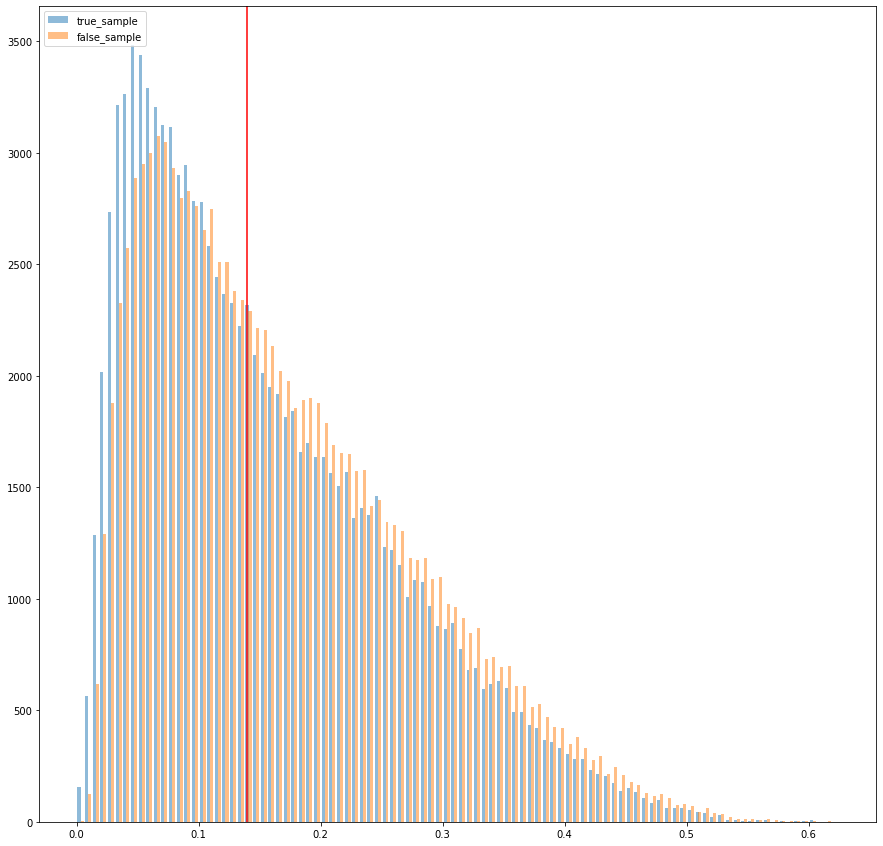
\includegraphics[width=0.43\linewidth]{images/Init-CelebA-Hist.png}}
    \qquad
    \subfloat[Result from ArcFace \label{fig:hist_arcface}]{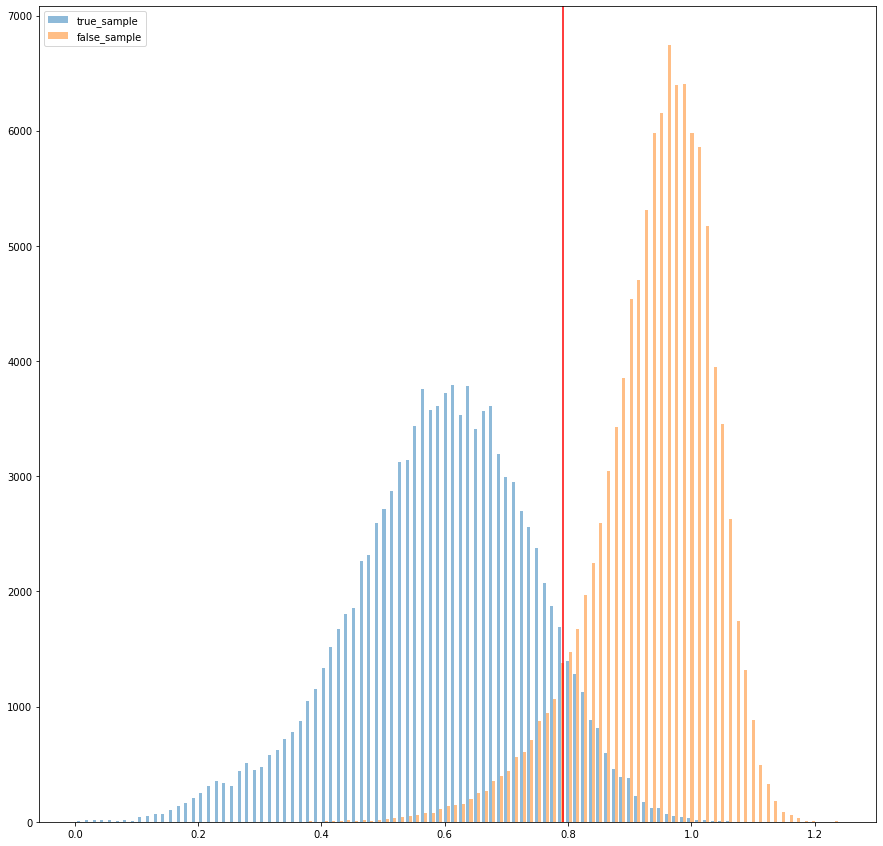
\includegraphics[width=0.43\linewidth]{images/ArcFace-CelebA-Hist.png}} 
    \quad 
    \subfloat[Result from LMCot \label{fig:hist_lmcot}]{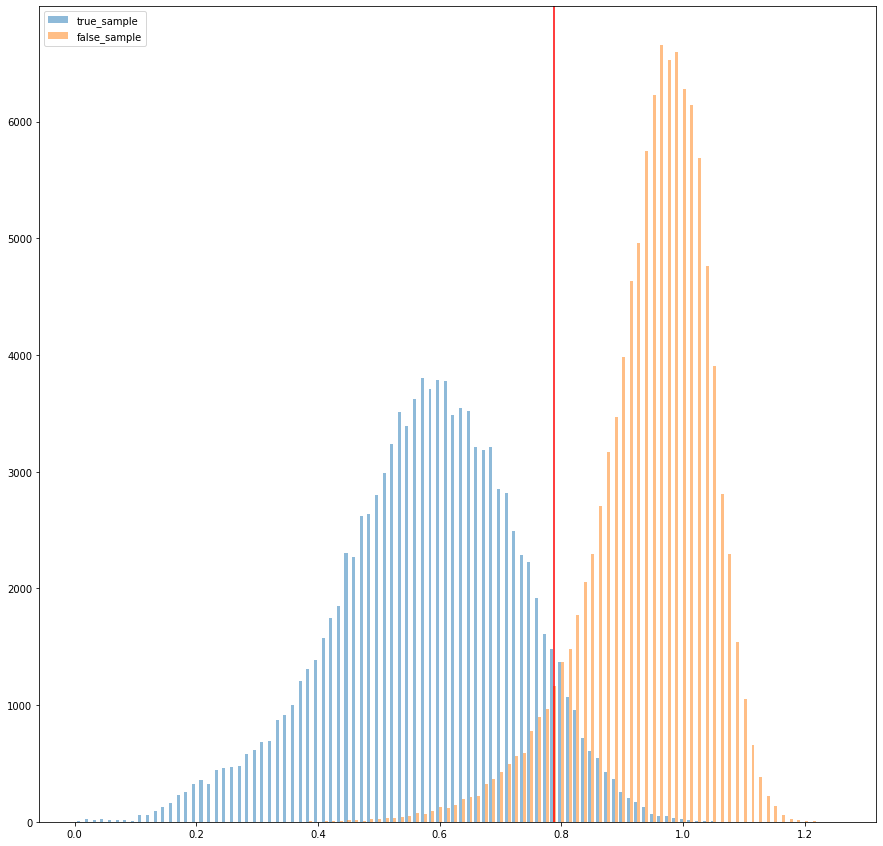
\includegraphics[width=1\linewidth]{images/LMCot-CelebA-Hist.png}}
    \caption{Cosine distances distribution of 100k random positive pairs and 100k random negative pairs from the CelebA test set. The blue part is positive pairs distance and the orange part is negative pairs distance. The red line shows the value at which the False Acceptance Rate (FAR) equals the False Rejection Rate (FRR). Figure (\ref{fig:hist_init}), (\ref{fig:hist_arcface}), and (\ref{fig:hist_lmcot}) illustrate the cosine distances distribution from the pretrained-weight on ImageNet, from a model trained with ArcFace and LMCot respectively.}
    \label{figure03}
\end{figure}

To check the feature extraction's performance of the model by the attributes, we use the Principal Component Analysis \cite{wold1987principal} (PCA) method to decompose the feature into two components. After training the model, it is possible to temporarily separate the attributes of the two opposite parts, such as male or female, black hair or not, double chin or not, etc.
\begin{figure}
    \centering
    \subfloat[Result from pretrained-weight on ImageNet \label{fig:pca_init}]{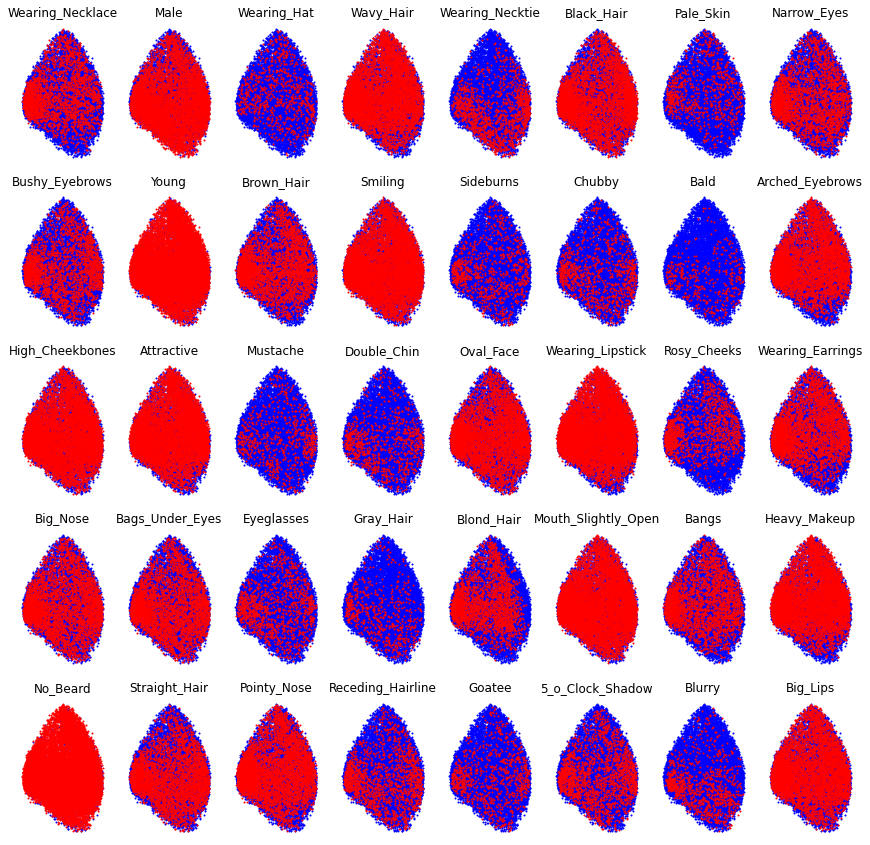
\includegraphics[width=0.42\linewidth]{images/Init-Face-Feature.png}} 
    \qquad
    \subfloat[Result from ArcFace \label{fig:pca_arcface}]{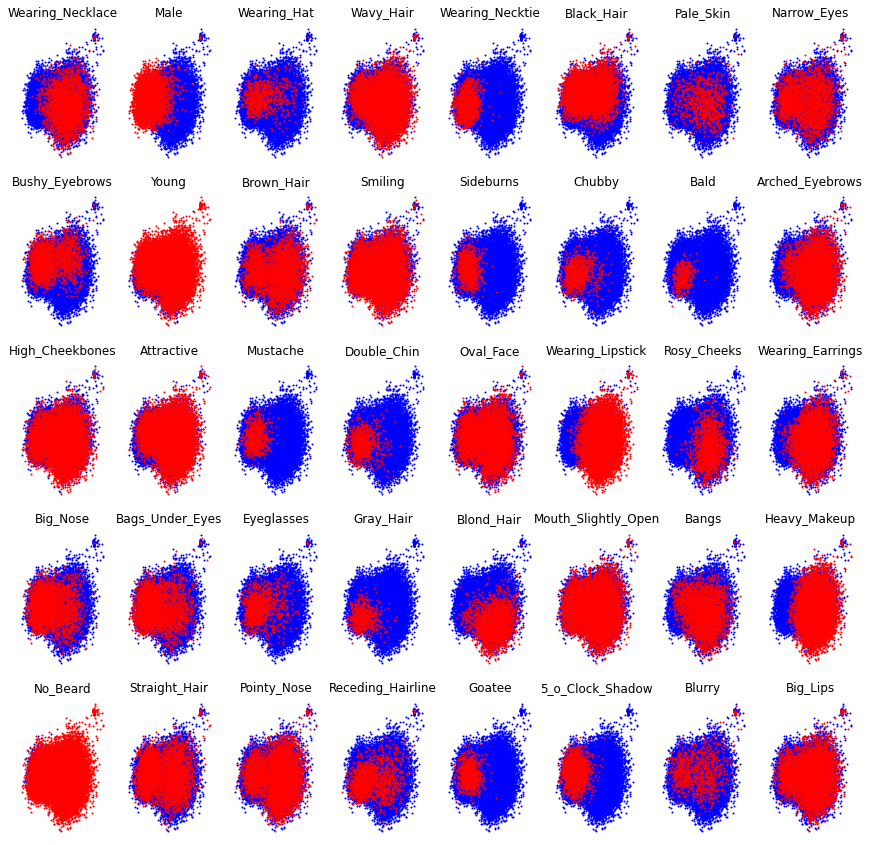
\includegraphics[width=0.42\linewidth]{images/ArcFace-Face-Feature.png}} \quad 
    \subfloat[Result from LMCot \label{fig:pca_lmcot}]{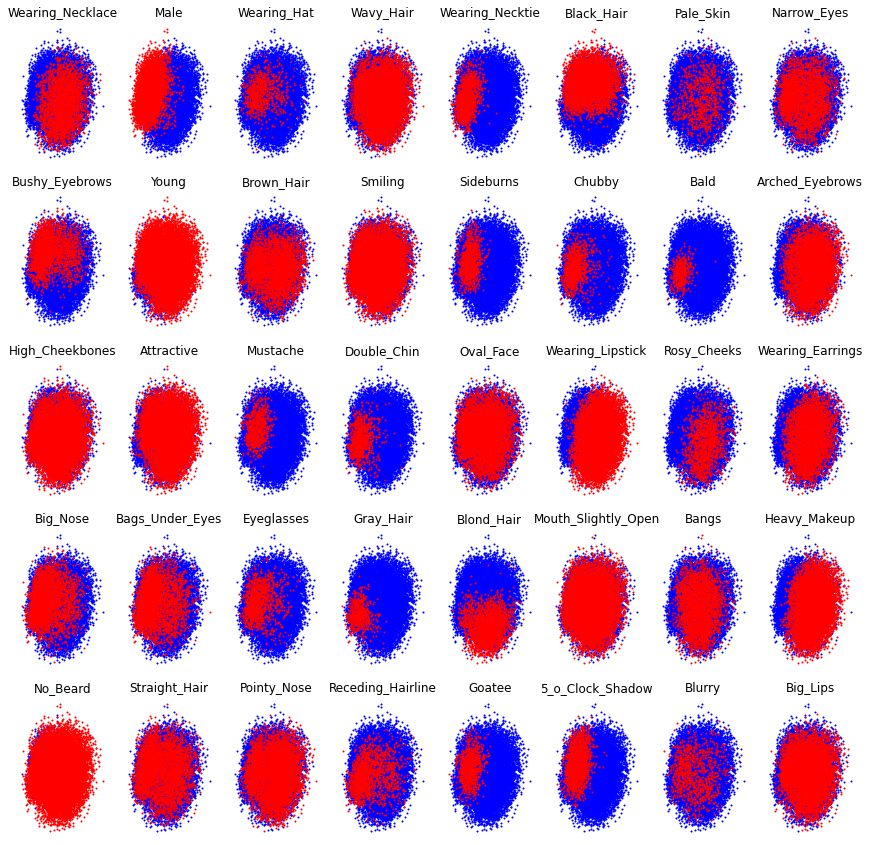
\includegraphics[width=\linewidth]{images/LMCot-Face-Feature.png}}
    \caption{We use PCA method to decompose feature into two components and plot with 40 attributes from CelebA test set. The red points represent the positive side of the feature and the blue points represent the negative side of the feature. Figure (\ref{fig:pca_init}), (\ref{fig:pca_arcface}), and (\ref{fig:pca_lmcot}) illustrate the distribution of 40 attributes from pretrained-weight on ImageNet, on model trained with ArcFace and LMCot respectively.}
    \label{figure04}
\end{figure}

\subsection{Speaker Verification (VLSP2021)} \label{s52}
The VLSP2021 Speaker Verification competition was held at the 8\textsuperscript{th} International Workshop on Vietnamese Language and Speech Processing. Focus on developing SV models with limited data. The provided training set has over 1000 speaker identities, and the competition consists of two relevant tasks:
\begin{itemize}
    \item \textbf{SV-T1}: Test set combines in-domain speakers and out-domain speakers.
    \item \textbf{SV-T2}: All speakers are external to the training dataset.
\end{itemize}

The performance of the models will be evaluated by the Equal Error Rate (EER) where the False Acceptance Rate (FAR) equals the False Rejection Rate (FRR). The evaluation metric is cosine similarity of the enrollment utterance and the test utterance.

In this competition, each participant has five submissions for each task. We experimented ResNet50 \cite{He2016DeepRL}, EfficientNetB0 \cite{tan2019efficientnet} as a backbone model, then add padding to the recordings to match the length of the longest recording. We used librosa \cite{mcfee2015librosa} to plot Mel Spectrograms of these audios with a default parameter, then fed it into the backbone model. Training data is split into five folds, four for training and one for validation. In the end, the model weight that has the best ERR on the validation set will be chosen. Finally, we ensemble all these weights by a mean score of each sample on the test set. By using this simple method, we achieved the following results:
\begin{table}[htbp]
\caption{Results on VLSP2021}
\label{table03}
\centering
\begin{threeparttable}
    \begin{tabular}{|l|l|l|}
    \hline
                        & SV-T1          & SV-T2           \\ \hline
    R50 + ArcFace       & 10.520         & 19.850          \\ \hline
    B0 + ArcFace        & 10.365         & 12.665          \\ \hline
    R50 + LMCot (ArcFace-based)        & 10.270         & 12.840          \\ \hline
    \textbf{B0 + LMCot (ArcFace-based)} & \textbf{9.215} & \textbf{12.535} \\ \hline
    Ensemble all        & 8.805          & 11.605          \\ \hline
    \end{tabular}
    
    \begin{tablenotes}
      \small
      \item Equal Error Rate (\%) on Speaker Verification (VLSP2021) competition. R50 is ResNet50 and B0 is EfficientNetB0. In the last row, we ensembled all 4 above results by mean with the same weight.
    \end{tablenotes}
\end{threeparttable}
\end{table}

\subsection{Google Landmark Retrieval 2021} \label{s53}
The 4\textsuperscript{th} Landmark Retrieval competition is one of the Instance-Level Recognition (ILR) workshop challenges at the International Conference on Computer Vision 2021 (ICCV 2021). In this competition, the developed models are expected to retrieve relevant database images to a given query image.

In this competition we use Google Landmark Dataset v2 \cite{weyand2020google} (gldv2) as dataset. These names are used for the following subsets of gldv2 \cite{henkel2021efficient}:
\begin{itemize}
    \item \textbf{gldv2}: 5M images of 200k classes.
    \item \textbf{gldv2c}: cleaned subset (1.6M images of 81k classes).
    \item \textbf{gldv2x}: non-cleaned subset restricted to only 81k classes, same as gldv2c (3.2M images).
\end{itemize}

Submissions are evaluated according to the mean Average Precision at 100, commonly referred to as (mAP@100):
\begin{equation}
\label{equation08}
    m A P @ 100=\frac{1}{Q} \sum_{q=1}^{Q} \frac{1}{\min \left(m_{q}, 100\right)} \sum_{k=1}^{\min \left(n_{q}, 100\right)} P_{q}(k) \operatorname{rel}_{q}(k)
\end{equation}
where $Q$ is the number of query images, ${{m}_{q}}$ is the number of index images containing a landmark in common with the query image $q$. ${{n}_{q}}$ is the number of predictions made by the system for query $q$, ${{P}_{q}}\left( k \right)$ is the precision at rank $k$ for the q-th query and $re{{l}_{q}}\left( k \right)$ is 1 if the k-th prediction is correct, and is 0 otherwise.

% The competition was held from August 11, 2021 to October 2, 2021. During the contest period, each team has a maximum of 5 submissions per day. For each submission, the system will show the public score. On the last day of the competition, each team is allowed to choose 2 submissions, and these 2 submissions will be counted towards the ranking results. Both public and private subset are hidden. Participants submit code on Kaggle. The system will run that code, and output the scores. Each inference submission should not exceed 12 hours run-time one CPU or GPU (Tesla V100).

We won the silver medal in this competition by using LMCot, despite the limited resources on hardware.

\begin{table}[htpb]
\centering
\caption{Results on Google Landmark Retrieval 2021}
\begin{threeparttable}
\begin{tabular}{|l|l|l|}
\hline
                                                                                                                        & Public           & Private          \\ \hline
\rowcolor[HTML]{C5E0B3} 
DELG (Baseline)                                                                                                         & 0.21480          & 0.22152          \\ \hline
4*B0-ArcFace   (Public)                                                                                                 & 0.24890          & 0.26164          \\ \hline
\rowcolor[HTML]{B4C6E7} 
\textbf{4*B0-LMCot (Ours)}                                                                                              & \textbf{0.26146} & \textbf{0.28338} \\ \hline
4*B7-ArcFace   (Public)                                                                                                 & 0.31940          & 0.32955          \\ \hline
\rowcolor[HTML]{B4C6E7} 
\textbf{4*B7-LMCot (Ours)}                                                                                              & \textbf{0.32476} & \textbf{0.34691} \\ \hline
4*V2M-ArcFace   (Ours)                                                                                                  & 0.32554          & 0.33973          \\ \hline
\rowcolor[HTML]{B4C6E7} 
\textbf{4*V2M-LMCot (Ours)}                                                                                             & \textbf{0.34933} & \textbf{0.36649} \\ \hline
ViT-ArcFace   (Ours)                                                                                                    & 0.35127          & 0.36569          \\ \hline
\rowcolor[HTML]{B4C6E7} 
\textbf{ViT-LMCot (Ours)}                                                                                               & \textbf{0.35720} & \textbf{0.36723} \\ \hline
\begin{tabular}[c]{@{}l@{}}ViT-ArcFace + ViT-LMCot \\ + B7-ArcFace + B7-LMCot \\ + V2M-LMCot + 2*V2S-LMCot\end{tabular} & 0.37283          & 0.38798          \\ \hline
\end{tabular}
    
    \begin{tablenotes}
      \small
      \item Results in Google Landmark Retrieval 2021 competition. B0 is EfficientNetB0\cite{tan2019efficientnet}, B7 is EfficientNetB7\cite{tan2019efficientnet}, ViT is Vision Transformer \cite{dosovitskiy2020image}, V2S is EfficientNetV2S\cite{tan2021efficientnetv2}, V2M is EfficientNetV2M\cite{tan2021efficientnetv2}. Submissions are evaluated according to the mean Average Precision at 100 (equation (\ref{equation08})). All LMCot solutions we used are built upon ArcFace.
    \end{tablenotes}
\end{threeparttable}
\end{table}

With a similar backbone model and training seed, LMCot gives better results than ArcFace. All results were trained using Google Colab Tensor Processing Unit (TPU) \cite{jouppi2017datacenter}. Hence, the results are reproducible. For models using ArcFace, to be most objective, we use results from public notebooks of other participants in this competition (if possible). All models are trained and inference on the same image size [256,256,3]. And all models trained by gldv2c are packed in TFRecord format.

Dieter's 1\textsuperscript{st} place solution [21] is very complex, combining many large models. Consequently, the result is outstanding by 0.51779 for the public score and 0.53751 for the private score. They trained 10 epochs on gldv2c (image size 224x224). After that, they trained 30-40 epochs on gldv2x (image size 512x512). Lastly, a few epochs on gldv2x of size 768x768. The models used are:

\begin{itemize}
    \item DOLG-EfficentNet-B5 (768x768) \cite{yang2021dolg}
    \item DOLG-EfficentNet-B6 (768x768) \cite{yang2021dolg}
    \item DOLG-Efficentnet-B7 (448x448) stride 1 \cite{yang2021dolg}
    \item Hybrid SwinBase224-EfficentNet-B5 (896x896) \cite{liu2021swin}
    \item Hybrid SwinBase224-EfficentNet b3 (896x896) \cite{liu2021swin}
    \item Hybrid SwinBase384-EfficentNet b6 (384,384) stride 1 \cite{liu2021swin}
    \item $3^{rd}$ place GLRec2020 EfficientNet-B6 (512x512) \cite{ha2020google}
    \item $2^{nd}$ place GLRec2020 EfficientNet-B5 (768x768) \cite{shubin2020google}
\end{itemize}

Models used by top teams are also very complicated and expensive which require a tremendous amount of GPU resources, such as from 2\textsuperscript{nd} place team \cite{yuqi20212nd} and 3\textsuperscript{rd} place team \cite{ha2021google}.

\subsection{Google Landmark Recognition 2021} \label{s54}
This is also one of the Instance-Level Recognition (ILR) workshop challenges at the International Conference on Computer Vision 2021 (ICCV 2021). This competition requires Kagglers to build correct landmark recognition models (if any) to evaluate challenging test images. Not surprisingly, cotangent consistently outperformed cosine in all tests.

In this competition, gldv2 is also used \cite{weyand2020google} as the training dataset. And submissions are evaluated by Global Average Precision (GAP) at (k), where (k=1)
\begin{equation}
\label{equation09}
    GAP=\frac{1}{M} \sum_{i=1}^{N} P(i) \operatorname{rel}(i)
\end{equation}

where $N$ is the total number of predictions returned from the judging system across all queries. At least one landmark in the total number of queries from the training set visible in it is $M$, some queries may not depict landmarks. $P$ and $rel$ are the same as Google Landmark Retrieval 2021 metric.

Despite the limited resources on hardware, we also won the silver medal in this competition.

\begin{table}[htpb]
\centering
\caption{Results on Google Landmark Recognition 2021}
\begin{threeparttable}
\begin{tabular}{|l|l|l|}
\hline
                                                                                                                          & Public           & Private          \\ \hline
\rowcolor[HTML]{C5E0B3} 
DELG (Baseline)                                                                                                           & 0.20245          & 0.19975          \\ \hline
4*B0-ArcFace   (Public)                                                                                                   & 0.21898          & 0.21468          \\ \hline
\rowcolor[HTML]{B4C6E7} 
\textbf{4*B0-LMCot (Ours)}                                                                                                & \textbf{0.22460} & \textbf{0.22242} \\ \hline
4*B7-ArcFace   (Public)                                                                                                   & 0.27760          & 0.26292          \\ \hline
\rowcolor[HTML]{B4C6E7} 
\textbf{4*B7-LMCot (Ours)}                                                                                                & \textbf{0.29926} & \textbf{0.29038} \\ \hline
4*V2M-ArcFace   (Ours)                                                                                                    & 0.28593          & 0.29134          \\ \hline
\rowcolor[HTML]{B4C6E7} 
\textbf{4*V2M-LMCot (Ours)}                                                                                               & \textbf{0.29963} & \textbf{0.29353} \\ \hline
ViT-ArcFace   (Ours)                                                                                                      & 0.30309          & 0.30480          \\ \hline
\rowcolor[HTML]{B4C6E7} 
\textbf{ViT-LMCot (Ours)}                                                                                                 & \textbf{0.30225} & \textbf{0.30605} \\ \hline
\begin{tabular}[c]{@{}l@{}}ViT-ArcFace +   ViT-LMCot \\ + B7-ArcFace + B7-LMCot \\ + V2M-LMCot + 2*V2S-LMCot\end{tabular} & 0.30900          & 0.31503          \\ \hline
\end{tabular}

    \begin{tablenotes}
      \small
      \item Results in Google Landmark Recognition 2021 competition. B0 is EfficientNetB0 \cite{tan2019efficientnet}, B7 is EfficientNetB7 \cite{tan2019efficientnet}, ViT is Vision Transformer \cite{dosovitskiy2020image}, V2S is EfficientNetV2S \cite{tan2021efficientnetv2}, V2M is EfficientNetV2M \cite{tan2021efficientnetv2}. Submissions are evaluated according to the mean Global Average Precision at $k=1$ (equation (\ref{equation09})). All LMCot we used is built on top of Arcface, replacing cosine with cotangent.
    \end{tablenotes}
\end{threeparttable}
\end{table}

Due to the restricted hardware with GPU-configuration limitation, we could not experiment larger models, in contrast to some complex solutions from 1\textsuperscript{st} place team \cite{henkel2021efficient}, $2^{nd}$ place team \cite{shubin20212nd} and $3^{rd}$ place team \cite{xu20213rd}.